\documentclass[11pt, oneside]{article}   	% use "amsart" instead of "article" for AMSLaTeX format
\usepackage{geometry}                		% See geometry.pdf to learn the layout options. There are lots.
\geometry{letterpaper}                   		% ... or a4paper or a5paper or ... 
%\geometry{landscape}                		% Activate for for rotated page geometry
%\usepackage[parfill]{parskip}    		% Activate to begin paragraphs with an empty line rather than an indent
\usepackage{graphicx}				% Use pdf, png, jpg, or eps� with pdflatex; use eps in DVI mode
								% TeX will automatically convert eps --> pdf in pdflatex		
\usepackage{amssymb}
\usepackage{amsmath}
\usepackage{parskip}
\usepackage{color}
\usepackage{hyperref}

\title{Curvature}
%\author{The Author}
%\section{}
%\subsection*{}
\date{}							% Activate to display a given date or no date

\graphicspath{{/Users/telliott_admin/Dropbox/Tex/png/}}
% \begin{center} 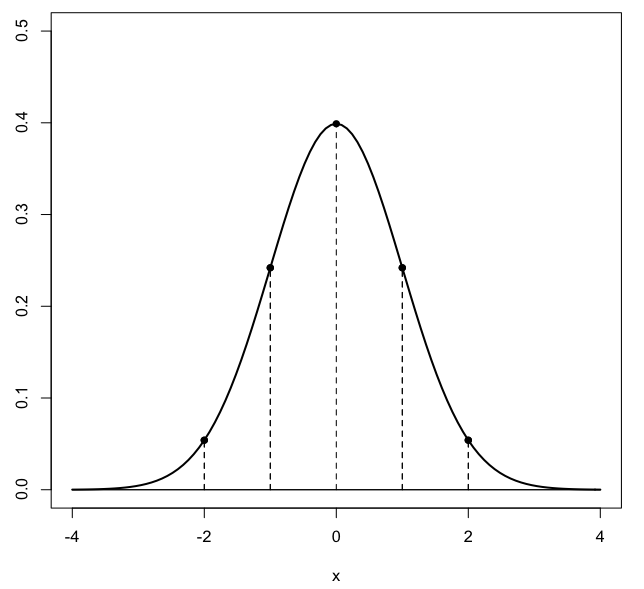
\includegraphics [scale=0.4] {gauss3.png} \end{center}
\begin{document}
\maketitle
\Large

We seek to expressions for curvature.  Consider two circles of differing radius.  We choose our measure of curvature $\kappa$ to be larger for the circle of smaller curvature.  That is, $\kappa \approx 1/R$.  For a path in space the "radius" of the curve followed can vary continuously.

The first definition says:  suppose that a particle moves with unit speed.  Then 
\[ \kappa = \frac{d}{dt} \ \mathbf{\hat{T}} \]

The first example is uniform circular motion on a circle of radius $R$.  We have 
\[ \mathbf{r}(t) = \langle x(t), y(t) \rangle \]
\[ = \langle R \cos \omega t, R \sin \omega t \rangle \]
The velocity is 
\[ \frac{d}{dt} \ \mathbf{r} = \mathbf{r}' = \omega R \langle - \sin \omega t, \cos \omega t \rangle \]
The speed squared is 
\[ | \mathbf{v} | ^2 = \omega^2 R^2 ((- \sin \omega t)^2 + \cos^2 \omega t ) = \omega^2 R^2 \]
so the speed is
\[ v = | \mathbf{v} | = \omega R \]
and it's a unit speed if we set $\omega = 1/R$.  So rewrite 
\[ \mathbf{r} = \langle R \cos \frac{t}{R}, R \sin \frac{t}{R} \rangle \]
\[ \mathbf{v} = \langle - \sin \frac{t}{R}, \cos \frac{t}{R} \rangle \]

The tangent vector $\mathbf{\hat{T}}$ is a unit vector in the same direction as the velocity.  Since we have set the speed to be unit speed
\[ \mathbf{\hat{T}} = \mathbf{v} = \langle - \sin \frac{t}{R}, \cos \frac{t}{R} \rangle \]
Recalling the definition
\[ \kappa = \frac{d}{dt} \ \mathbf{\hat{T}} \]
we see that $\kappa$ is just the acceleration, namely
\[ \kappa = | \mathbf{a} | = | \mathbf{v}' | \]
\[ = | -\frac{1}{R} \langle \cos \frac{t}{R}, \sin  \frac{t}{R} \rangle | \]
\[ = \frac{1}{R} \]

For an arbitrary curve (not necessarily unit speed)
\[ \kappa = \frac{ | \mathbf{\hat{T}}' |}{| \mathbf{r}' |} \]

Problem:  find the curvature of the parabola $y=x^2$ at the point $(1,1)$.

First, we can parametrize the curve as 
\[ \mathbf{r}(t) = \langle t, t^2 \rangle \]
with the corresponding $t$ for $(1,1)$ equal to $1$.
Then
\[ \mathbf{r}' = \langle 1, 2t \rangle  \]
\[ | \mathbf{r}' | = \sqrt{1 + 4t^2} \]

And
\[ \mathbf{\hat{T}} = \frac{\mathbf{v}}{| \mathbf{v} |} =  \frac{\mathbf{r}'}{| \mathbf{r}' |} \]
We have
\[ \frac{\mathbf{r}'}{| \mathbf{r}' |} = \frac{1}{\sqrt{1 + 4t^2}} \ \langle 1, 2t \rangle \]
\[ =  \langle \frac{1}{\sqrt{1 + 4t^2}}, \frac{2t}{\sqrt{1 + 4t^2}} \rangle \]
So
\[ \mathbf{\hat{T}}' = \frac{d}{dt} \  \frac{\mathbf{r}'}{| \mathbf{r}' |} \]
\[ =  \langle -4t (1+4t^2)^{-3/2}, ?? \rangle \]
We need the derivative:
\[ \frac{d}{dt} \ \frac{2t}{\sqrt{1 + 4t^2}} = \frac{2 \sqrt{1+4t^2} + 8 t^2(1+4t^2)^{-3/2}}{1+4t^2} \]
\[ = \frac{2}{\sqrt{1+4t^2}} + 8t^2 (1+4t^2)^{-5/2} \]

What a mess!  We need to find the length of this thing and then divide by $|\mathbf{r}|$ but life is too short for that.

\end{document}  